%
%
\subsection*{TODO list}
{\color{red}
\begin{description}
\item[Sensitivity plots.] 	
 Create plots for the CPV and HM sensitivities for 40kton detector and 1.2 MW beam. Plots should include various combinations of the assumed uncertainties: with current best measurements,  with best guesses about uncertainties we can archive and with  uncertainties which will be obtain using beam test experiment at CERN.
\item[E-m shower calibration energy scale.] 
Estimate statistics of particles to optimise the measurement of EM showers.  Provide the necessary statistics  as a function of energy. Optimise the energy bins widths, where we expect coarser bins for higher energies than for lower energies.    

\item[Hadronic shower calibration] 
Estimate statistics of particles to optimise the measurement of hadronic showers.  Provide the necessary statistics as a function of energy. Optimise the energy bins widths, were we expect coarser bins for higher energies than for lower energies.    \\
Estimate pi0 production from the proton scattering in the TPC. 
\item[Reconstruction issues.] 
Obtain values for the uncertainties due to finding vertex position of neutrino interactions. \\
Estimate statistics necessary to improve low energy electrons acceptance due to reconstruction algorithms limitations. 
\item[e/gamma separation] 
Estimate statistics necessary  for improvement of the e/gamma separation.  Assume three values for wire pitch: 3mm,  4mm and 5mm.
\item[Pion cross sections: absorption, charge exchange in Ar] 
Get statistics for pions to measure their cross sections. Estimate energy bin widths.
\item[Kaon cross section in Ar] 
Get statistics for kaons to measure their cross sections. Estimate energy bin widths.
\item[Muon capture] 
Estimate statistics for antimuons for capture on argon to be used for the statistical determination of the wrong sign neutrino contribution on the beam. 
\end{description}

}

\subsection{Requirements for the detector, beam and commissioning}
\label{detbeam_main}
The Single-Phase Cern Prototype detector is intended to provide necessary information to reduce systematic uncertainties for the oscillation measurements in the US-based long base-line neutrino experiment.   The LAr TPC technology is not new but wasn't extensively used in the 1-10 GeV neutrino energy range.  The main source of uncertainties due to detector with the current values are shown in table \ref{table:deterr}


\begin{table}[h]
\centering
\caption{Current known sources of detector uncertainties for liquid argon or TPC.}
\label{table:deterr}
\begin{tabular}{|c|c|c|}
\hline
\textbf{source of uncertainty } & \textbf{value} & \textbf{reference}  \\ \hline
  e/$\gamma$ separation        &           &                   \\ \hline
  e-m shower calibration        &           &            \\ \hline
   hadronic shower calibration       &           &        \\ \hline
low energy acceptance electron identification &   &  \\ \hline
 .....   &   &   \\ \hline
\end{tabular}
\end{table}



\begin{table}[h]
\centering
\caption{Current known sources of  uncertainties due to interaction of charged particle with argon.}
\label{table:physicserr}
\begin{tabular}{|c|c|c|}
\hline
\textbf{source of uncertainty } & \textbf{value} & \textbf{reference}  \\ \hline
 pion(Kaon) absorbtion       &           &                   \\ \hline
 pion(Kaon) charge exchange       &           &            \\ \hline
pion (Kaon) production in secondary interactions  &   &  \\ \hline
 muon capture       &           &  Phys. Rev. C 35, 2212      \\ \hline
energy scale  &   &   \\ \hline
Michel electron tagging  &  &  \\ \hline

 .....   &   &   \\ \hline
\end{tabular}
\end{table}



With current detector uncertainties from table \ref{table:deterr} the sensitivities for the CP violation phase measurement is shown in Fig. \ref{fig:cpsensitivity}  {\bf Task: make this plot} . The  proposed test beam detector will reduce uncertainties to XX\%  and improve our sensitivity to $\delta_{CP}$ as shown in Fig. \ref{fig:cpsensitivity} {\bf Task: make this plot.}



\begin{figure}[h!]
  \centering
%\includegraphics[scale=0.4]{}
\label{fig:cpsensitivity}
  \caption{Sensitivites for the $\delta_{CP}$ measurement  for using current knowledge of the single-phase LAr-TPC detector technology and for reduced detector uncertainties from SPCP beamtest data.  The plots prepared for 40 kton fiducial mass and $xx\times 10^{21}$POT.}
\end{figure}

\newpage

\subsubsection{Particles energy and direction}
\label{detbeam_particles}
Plans for running beam for the the ELBNF include both neutrino and anti-neutrino configurations. These beams will be composed  mainly of muon neutrinos (anti-neutrinos) as well as electron neutrinos (anti-neutrinos). In figures \ref{fig:particle_momenta} and \ref{fig:particle_theta} the distributions on momenta and angles of particles created in neutrino interaction are shown. 

\begin{figure}[h!]
  \centering
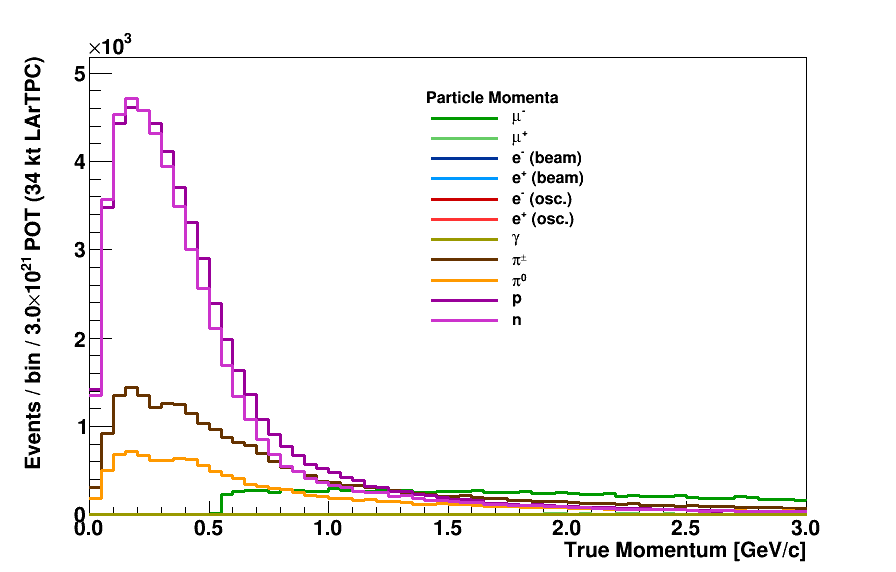
\includegraphics[scale=0.4]{figures/True_Momenta_per_Particle}
\label{fig:particle_momenta}
  \caption{Particle momenta distributions for particles coming from all fluxes ($\nu_e$, $\nu_\mu$, $\bar \nu_e$ and $\bar \nu_\mu$) at both near and far detector locations.  }
\end{figure}


\begin{figure}[h!]
  \centering
%\includegraphics[scale=0.4]{figures/True_Theta_per_Particle}
\label{fig:particle_theta}
  \caption{Particle angle wrt to the beam axis distributions for particles coming from all fluxes ($\nu_e$, $\nu_\mu$, $\bar \nu_e$ and $\bar \nu_\mu$) at both near and far detector locations.  }
\end{figure}

\newpage


\begin{figure}[htp]
  \centering
  \label{fig:containment}
  
  \begin{tabular}{ccc}
    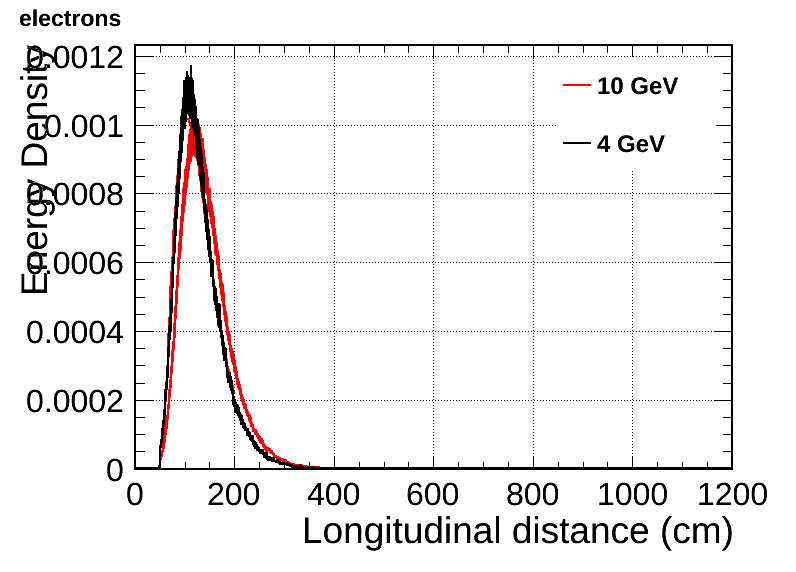
\includegraphics[scale=0.15]{figures/electrons_density_overlay}&
    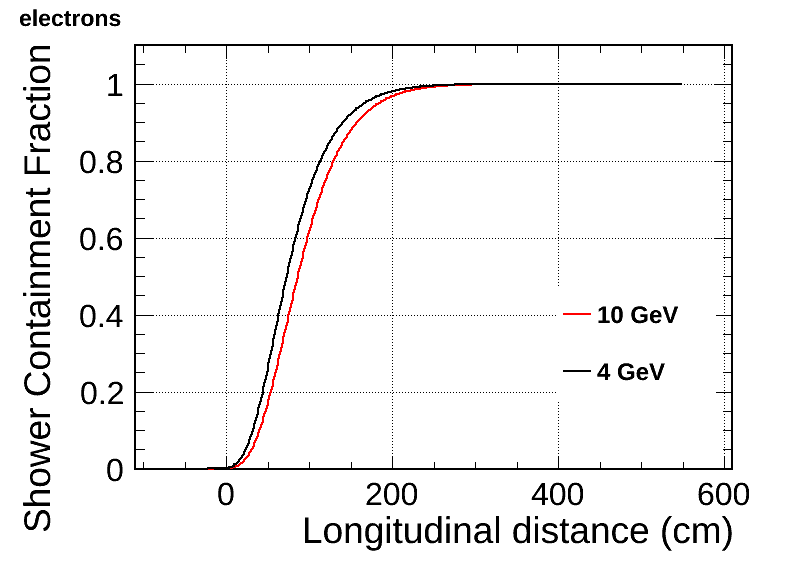
\includegraphics[scale=0.15]{figures/electrons_lcont_overlay}&
    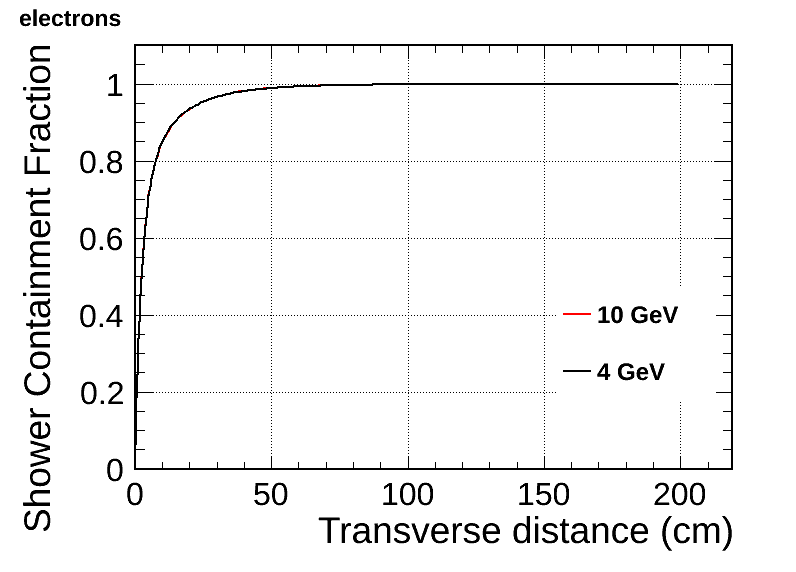
\includegraphics[scale=0.15]{figures/electrons_wcont_overlay}\\
 
 
    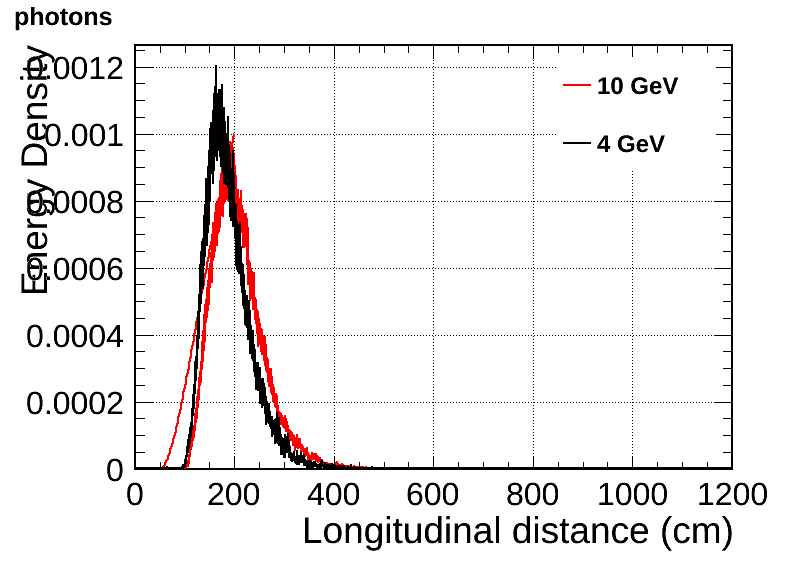
\includegraphics[scale=0.15]{figures/photons_density_overlay}&
    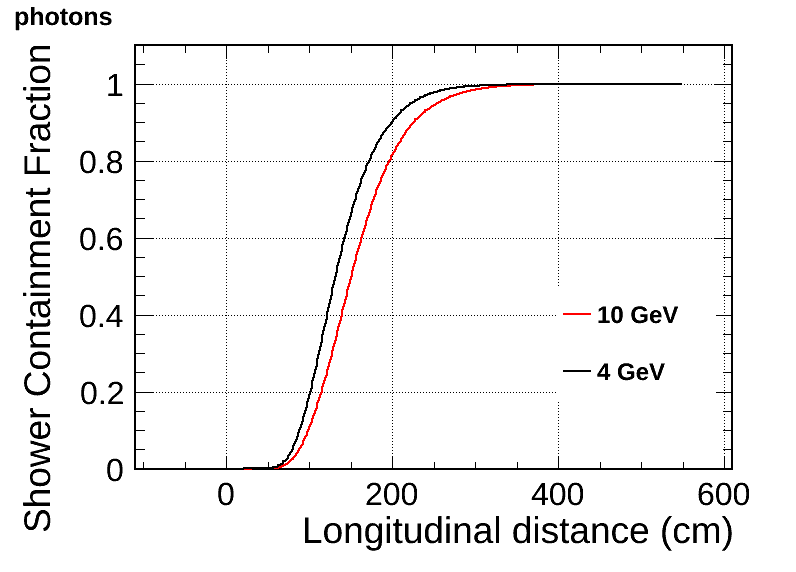
\includegraphics[scale=0.15]{figures/photons_lcont_overlay}&
    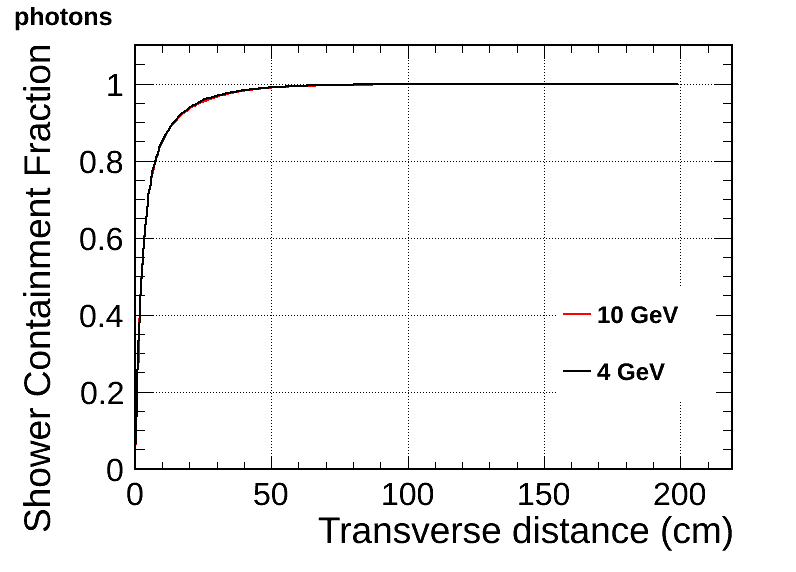
\includegraphics[scale=0.15]{figures/photons_wcont_overlay}\\
 

    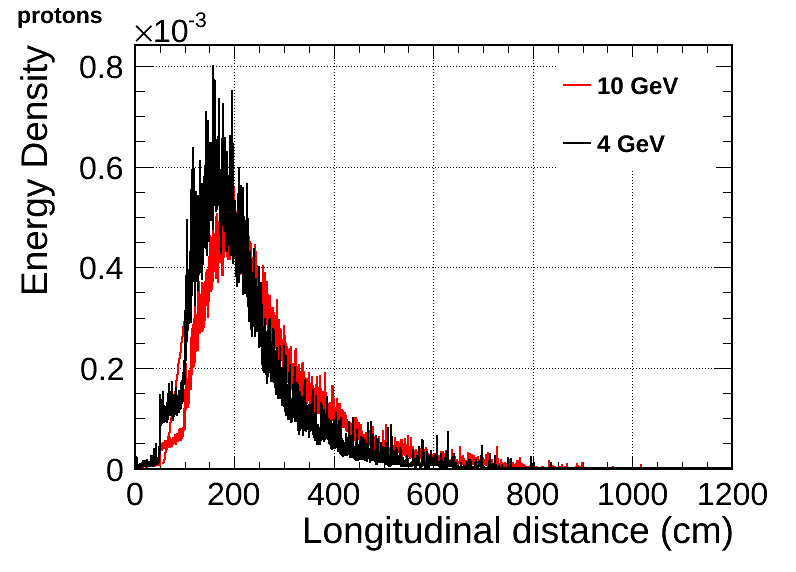
\includegraphics[scale=0.15]{figures/protons_density_overlay}&
    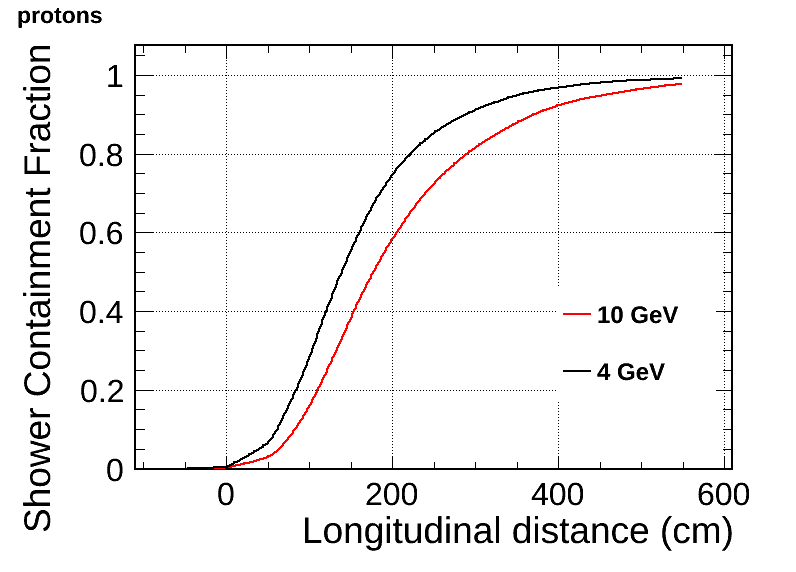
\includegraphics[scale=0.15]{figures/protons_lcont_overlay}&
    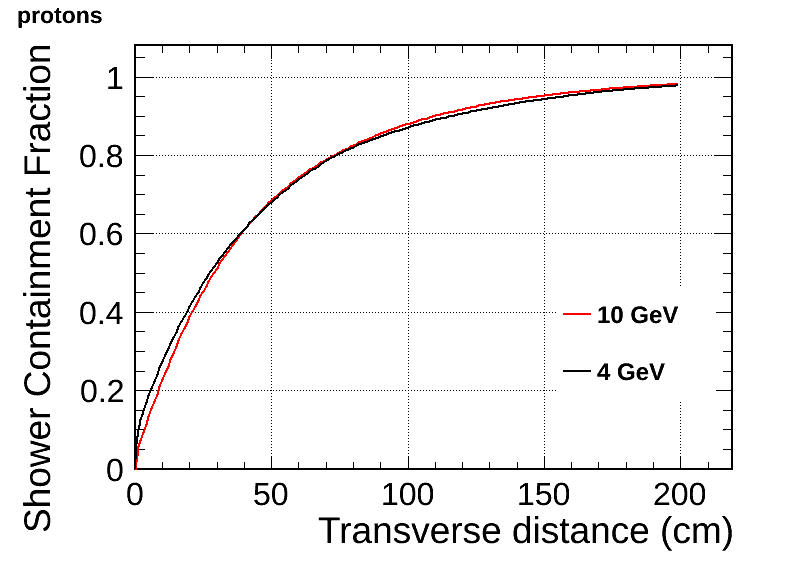
\includegraphics[scale=0.15]{figures/protons_wcont_overlay}\\
 
    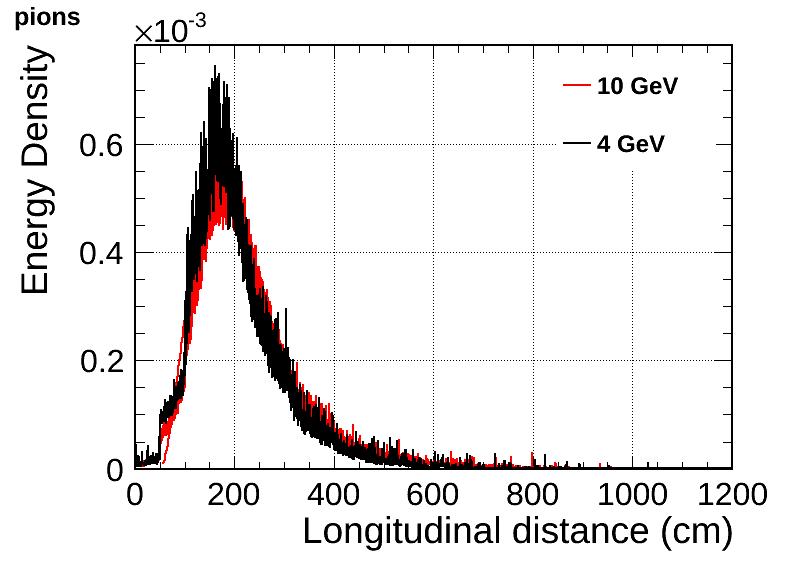
\includegraphics[scale=0.15]{figures/pions_density_overlay}&
    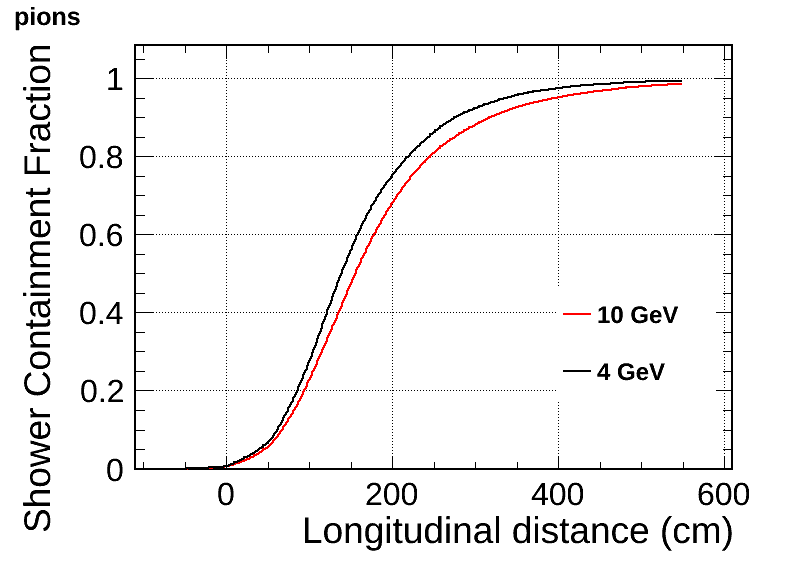
\includegraphics[scale=0.15]{figures/pions_lcont_overlay}&
    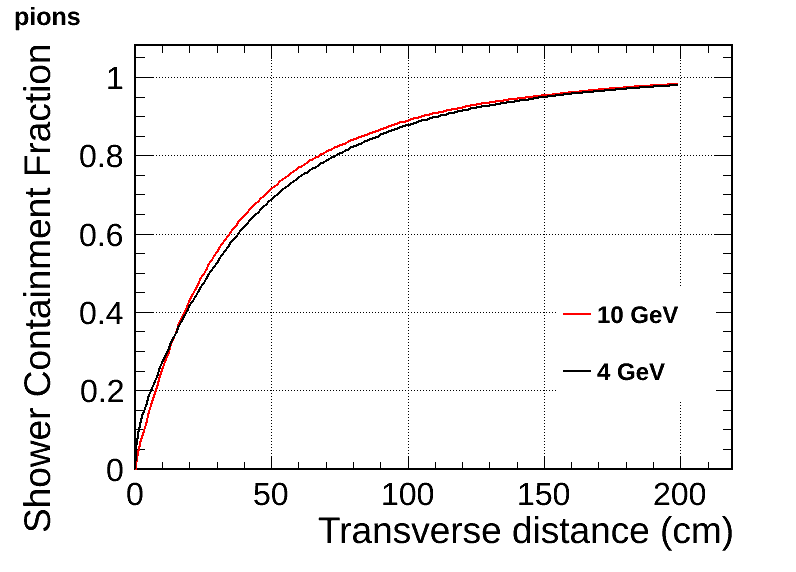
\includegraphics[scale=0.15]{figures/pions_wcont_overlay}\\
 
    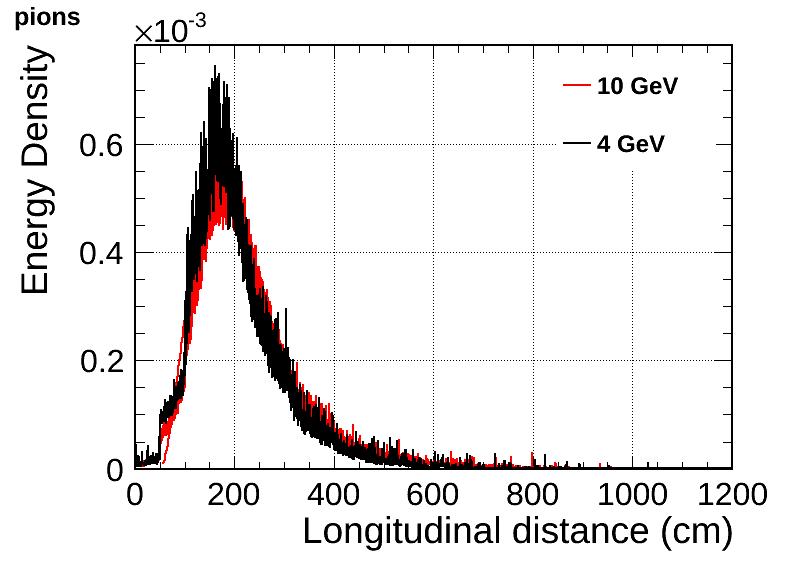
\includegraphics[scale=0.15]{figures/pions_density_overlay}&
    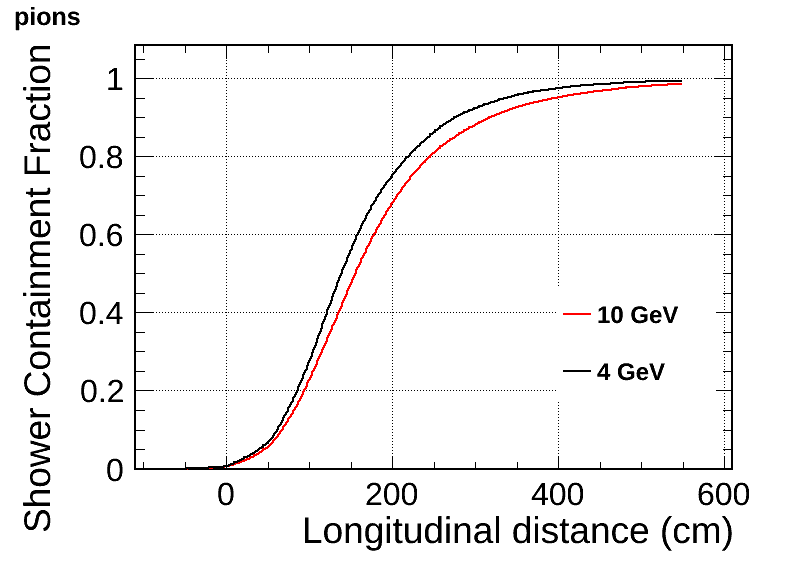
\includegraphics[scale=0.15]{figures/pions_lcont_overlay}&
    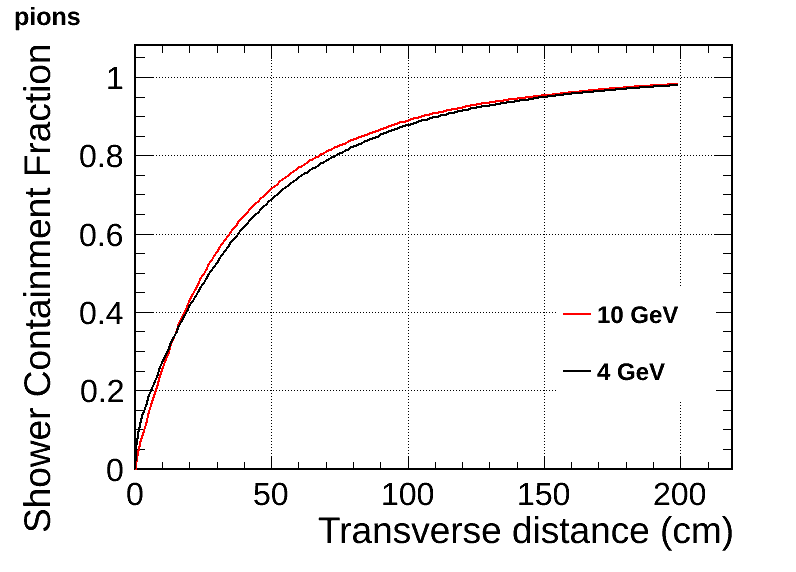
\includegraphics[scale=0.15]{figures/pions_wcont_overlay}\\
 
 
    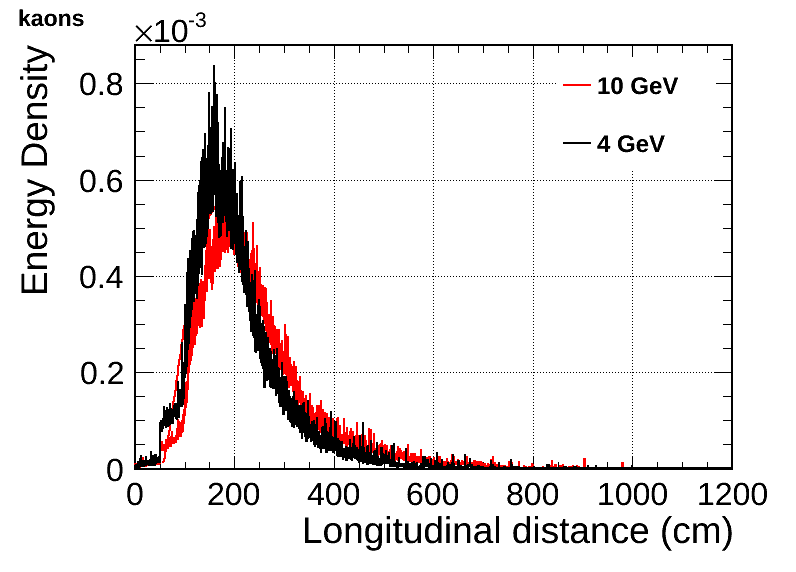
\includegraphics[scale=0.15]{figures/kaons_density_overlay}&
    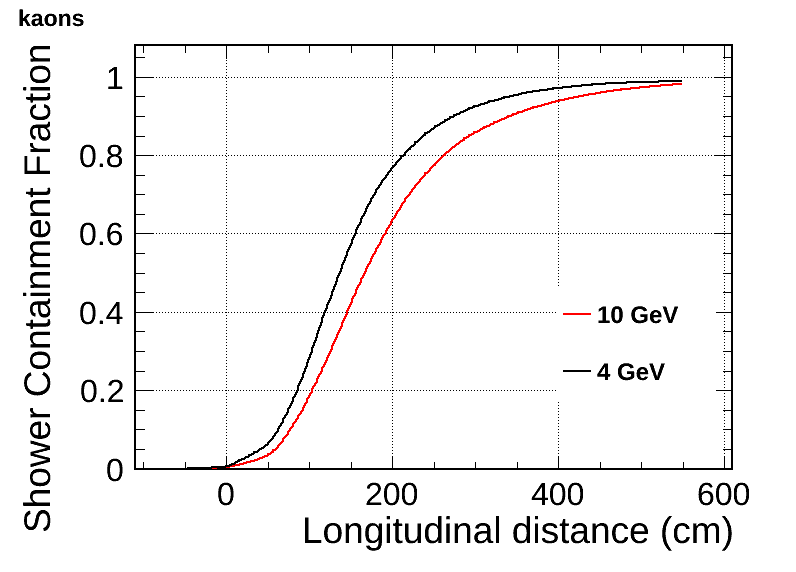
\includegraphics[scale=0.15]{figures/kaons_lcont_overlay}&
    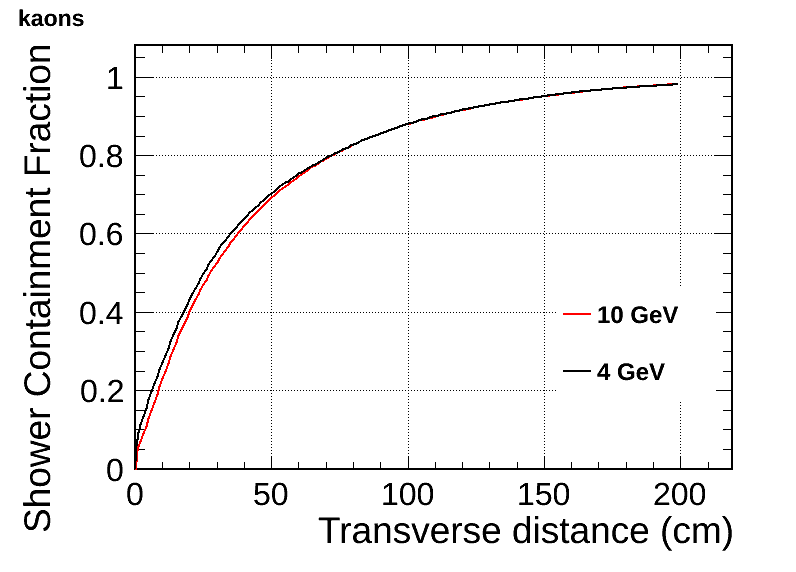
\includegraphics[scale=0.15]{figures/kaons_wcont_overlay}\\
 
  \end{tabular}
  \caption{Particle containment plots.}
\end{figure}

\clearpage
%\subsubsection{Particle rates}
%\label{detbeam_rates}
%Estimation of  beam particles rates  necessary to collect high enough statistics in a reasonable time to obtain goals of of the measurements.
% THis should be discussed in the beam section
\subsubsection {Run plan}

Table~\ref{tab:runplan} summarizes the required exposures to beam particles.
\begin{table}[h]
\centering
\begin{tabular}{|c|c|c|l|}
\hline
Particle & Momenta (GeV) & Exposure & Purpose \\ \hline
charged $\pi$       & 0.1, 0.2, 0.3, 0.4, 0.5, 1, 2, 3, 5, 10     &  10K  & hadronic shower \\ \hline
charged $\pi$ &  1  &  10K  & vary angle, reconstruction \\ \hline
electron       &    0.1, 0.2, 0.3, 0.4, 0.5, 1, 2, 3, 5, 10        &    100K   & EM shower/e-$\gamma$ PID     \\ \hline
electron &  1  &  10K  & vary angle, reconstruction \\ \hline
muon &   0.1, 0.3, 0.5, 1, 2, 5, 10  &  10K & $E_\mu$ calibration, MCS \\ \hline
muon &  1  &  10K  & vary angle, reconstruction \\ \hline
proton & 0.1, 0.2, 0.3, 0.5, 1, 2   &  10K & response, PID \\ \hline
proton &  1  &  10K & vary angle, reconstruction \\ \hline
kaon  & 0.1, 0.2, 0.3, 0.5, 1 & ?   &   response, PID  \\ \hline
\end{tabular}
\caption{Run plan requirements.}
\label{tab:runplan}
\end{table}

NUMBERS ARE UPDATED GUESSES - STUDIES NEEDED HERE \\
Charged pion samples will be used to characterize hadronic shower response and to measure
absorption cross section parameters on argon. NEED STUDY of HADRONIC SHOWER RESOLUTION
(for now pion statistics give better than $\sim$1\% measurement of mean for upper limit from 50\%/$\sqrt{E}$ in sampling calorimeters
for all energies except 0.1 GeV point). 
Muon samples will be used for calibration and 
reconstruction tests. Electron samples will be used to measure EM shower response  
and to tune PID algorithms (statistics shown will far exceed 1\% uncertainty on the mean for 
<<<<<<< HEAD
EM showers with resolution as measured in DOCDB 8848). 
=======
EM showers with resolution on the order of 1\% as measured in DOCDB 8848. 100k Electron event samples will allow
high statistics studies of e-gamma separation).  
>>>>>>> 126f122ef285efd0cadb8fa3d92b937255540fa6
Proton response will be studied for reconstruction and to tune PID 
algorithms. Kaon data will be needed to tune proton decay backgrounds .
Special runs at various angles with $\pi$, $\mu$, p and electrons will be performed to study reconstruction and tune PID algorithms. 

\subsection{Detector performance tests}

\subsubsection{Bethe-Bloch parametrisation of charged particles}

The SPCP will allow to study the detector response to charge particles from the test beam and will serve as a calibration detector. The measured energy deposition for various particles and its dependence on the direction of the particle will feed into our Monte Carlo generator and allow more precise reconstruction of neutrino energy and interactions topologies with good particle identifications.
 
{\bf How we compare with Lariat?} 
{\bf Multiple scattering}  

The set of single-phase prototype detector helped to understand the detector response to cosmic muons. But there is still lots to learn with additional studies. 
The charge  particle identification efficiencies  has been mapped for only limited range of the particle energies.  


\begin{table}[h]
\centering
\begin{tabular}{|c|c|c|}
\hline
Particle     & Momenta (GeV)                                                                                       & Exposure/bin (total)  \\ \hline
$\pi ^+ $   & 0.2-1.0 (50MeV bins), 1.0-3.0 ( 100MeV bins), 3.0-10 ( 200MeV bins)    &  200 (16.6k)     \\ \hline
$\pi ^- $    & 0.2-1.0 (50MeV bins), 1.0-3.0 ( 100MeV bins), 3.0-10 ( 200MeV bins)    &  200 (16.6k)     \\ \hline
$e^+$       & 0.2-10  (200MeV bins)                                                                              &  200 (9.8k)        \\ \hline
$e^- $       & 0.2-10  (200MeV bins)                                                                              &  200 (9.8k)        \\ \hline
$\mu^+$   & 0.2-1.0 (50MeV bins), 1.0-3.0 ( 100MeV bins), 3.0-10 ( 200MeV bins)    &  200 (16.6k)    \\ \hline
$\mu^-$    & 0.2-1.0 (50MeV bins), 1.0-3.0 ( 100MeV bins), 3.0-10 ( 200MeV bins)    &  200 (16.6k)     \\ \hline
$p$          &  0.2-1.5 (50MeV bins), 1.5-3.0 ( 100MeV bins), 3.0-10 ( 200MeV bins)    &  200 (17.2k)     \\ \hline
$\bar p$   &  0.2-1.5 (50MeV bins), 1.5-3.0 ( 100MeV bins), 3.0-10 ( 200MeV bins)    &  200 (17.2k)    \\ \hline
$K^+$      &  0.2-1.5 (50MeV bins), 1.5-3.0 ( 100MeV bins), 3.0-10 ( 200MeV bins)    &  200 (17.2k)      \\ \hline
$K^- $      &  0.2-1.5 (50MeV bins), 1.5-3.0 ( 100MeV bins), 3.0-10 ( 200MeV bins)    &  200 (17.2k)    \\ \hline
\end{tabular}\caption{Data sample requirments for the $dE/dx$ Bethe-Bloch parametrisation. The lower range starts with the nominal 200 MeV which is not achivable for p and dificult for K. The rough estimate is that we need about 200 particles per bin assuming that about half of them will be actually meareured it gives  1\% statistical error for each bin. About half of the data sample is in the high momenta region, which can be reduce by decresing number of particles per bin. }
\end{table}




\subsubsection{e/$\gamma$ separation}

The separation of the electrons from photons is the most important feature of the LAr TPC detectors for the search of the CP violation phase where we look for appearance of the $\nu_e$ in the $\nu_\mu$ beam.  Showers from electrons are part of the signal whilst the single photons might contribute to the background sample. The photons can undergo two process: pair production and Compton scattering. The dominant process for photons with energies of several hundreds MeV  is the e$^+$ e$^-$ pair production, but Compton scattering also occur at this energies. For pair production the e/$\gamma$ separation is achieved by looking at the beginning of the electromagnetic shower, where for election we see energy deposition typical for single MIP and for photon we see energy deposition consisted with two MIP. The separation of e/$\gamma$ has been measured in the ArgoNEUT experiment using neutrino scattering data with low statistics. Currently the separation efficiency is estimated to be at the level of of 94 \% (? cite and check the number). In case of Compton scattering off of atomic electrons the signal is much more difficult to distinguish from the CC $\nu_e$ scattering signal.

The separation of  the e/$\gamma$ measured by ArgoNEUT is not sufficient for the ELBNF experiment. Here we propose a measurement of the separation efficiency  as the function of energy and angle.  {\bf we need someone to look into this}



\subsubsection{Reconstruction efficiencies and particle identification}
\label{detbeam_pid}

The reconstruction of events in the LAr TPC is still a challenge but rapid progress has been achieved in recent years (cite pandora and other reconstruction algorithms). Despite the progress reconstruction algorithms have to rely Monte Carlo predictions which don't simulate liquid argon detectors responses correctly. Reconstruction algorithms will benefit greatly from test beam data particularly from the full scale prototype. The reconstruction algorithms will be trained to correctly reconstruct track, electromagnetic and hadronic showers.
The data of tracks and showers can be used to create a library of reference events with which to tune algorithms.
%which can be used for matching with he neutrino data, similar to the  LEM (library event matching).

Main issues for the reconstruction algorithms:
\begin{itemize}
\item The reconstruction algorithms try to use all three planes on the signal readout. if the orientation of the track/shower is such that it is aligned with wires on one of the plans it significantly reduces quality of reconstructed objects. 
\item Calorimetry with collection and induction planes. In the ICARUS experiment the deposited energy was reconstructed from the signal on the collection plane. The induction planes bipolar signal wasn't "stable" enough to use it for calorimetric measurement. In the ELBNF design there is additional shielding  wire plane which will improve the quality of the bipolar signal and the  test beam experiment will help with its calibration.
\item   Vertexing.
\item Reconstruction efficiency for low energy particles. The reconstruction algorithm suffer from the lose of fefficiency for low energy particle or particles which leave less than 200-300 hits. Training the algorithms on a low energy particles from the test beam will improve the quality and efficiency of the reconstructed objects.
\end{itemize}



\subsubsection{Cross section measurements}
Precise measurement of the  absorption and charge exchange of pions and kaons. Pion absorption is a large part of the pion nucleon cross section from 50 MeV to 500MeV with no data above about 1GeV pion kinetic energy. 
{\bf Add plots and values for known cross sections wit errors} 
\begin{itemize}
\item pion absorption on argon - Kotlinski, EPJ 9, 537 (2000)
\item pion cross section as a function of A - Gianelli PRC 61, 054615 (2000)
\end{itemize}
There is not currently a satisfactory theory describing absorption. The Valencia group (Vicente-Vacus NPA 568, 855 (1994)) developed model of    the pion-nucleus reaction with fairly good agreement, although not in detail. The actual  mechanism of multi-nucleon absorption
 is not well understood. 
 
\subsubsection{Charge sign determination}
It is not possible to determine charge of the particle on the event by event basis with non-magnetised LAr TPC detectors. A statistical separation will be studied which will make use of differences in muon versus antimuon capture cross sections and lifetime.
%However, the statistical analyst will be possible. We will fit the muon's half time which is different for muons and antimony due to different muon capture cross sections. 
For the $\mu^+$ for argon we expect about xx\% to be captured and for $\mu^-$ about yy\%. 

\subsubsection{Single track calibration}

\subsubsection{Shower calibration}

Reconstruction of neutrino energy depends of a quality of reconstruction of both electromagnetic and hadronic showers. 

- {\bf features of Hadronic shower in LAr TPC}
- {\bf features of electromagnetic shower in LAr TPC}
- Missing energy from neutral (Neutrons scattering)
 

\subsection{Other measurements} 
\subsubsection{Anti-proton annihilation }
\subsubsection{Proton decay background (cosmogenic $K^{0} \to K^+$)}



